\section{Implementierung}

\subsection{YOLOv5}
YOLO, ein Bilderkennungsmodell, wurde von Joseph Redmon und Ali Farhadi an der Universität von Washington entwickelt und im Jahr 2015 veröffentlicht. YOLO steht für "You Only Look Once", was darauf hinweist, dass das Modell nur einmal auf ein Bild schaut, um Objekte schnell und präzise zu erkennen. Seit seiner Veröffentlichung wurden insgesamt neun Versionen von YOLO veröffentlicht \cite{Yolo}.

Wir uns für ein vortrainiertes Modell der fünften Version von Yolo entschieden, das bereits für unsere spezifischen Anforderungen trainiert wurde. Obwohl wir mit der fünften Version eine ältere Version von YOLOv5 verwenden, bedeutet dies nicht, dass das Modell weniger effektiv ist. Für viele größen ist YOLOv5 etws schneller als zum Beispiel YOLOv8. Für uns ist die Geschwindigkeit wichtig, da wir das Model auf dem Raspberry Pi 4 laufen lassen und dort nicht viel Leistung haben.  Es kam uns daher auch zugute, das der Entwickler Yolov5s also ein kleineres Model von YOLO verwendet hat.   Der Entwickler des Modells hat Bilder aus verschiedenen Quellen gesammelt und ein eigenes benutzerdefiniertes Datenset erstellt, das aus 374 Trainingsbildern und 111 Validierungsbildern besteht.


\begin{figure}[H]
	\centering
	\begin{minipage}[b]{0.3\textwidth}
		\centering
		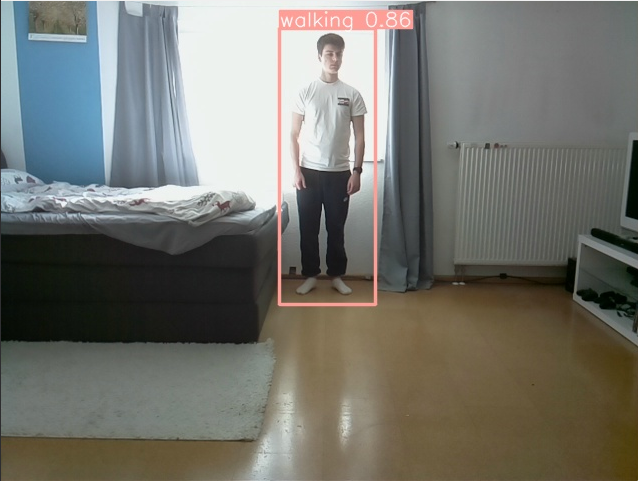
\includegraphics[width=\textwidth]{images/walking.png}
		\caption*{Klasse: ''walking''}
	\end{minipage}
	\hfill
	\begin{minipage}[b]{0.3\textwidth}
		\centering
		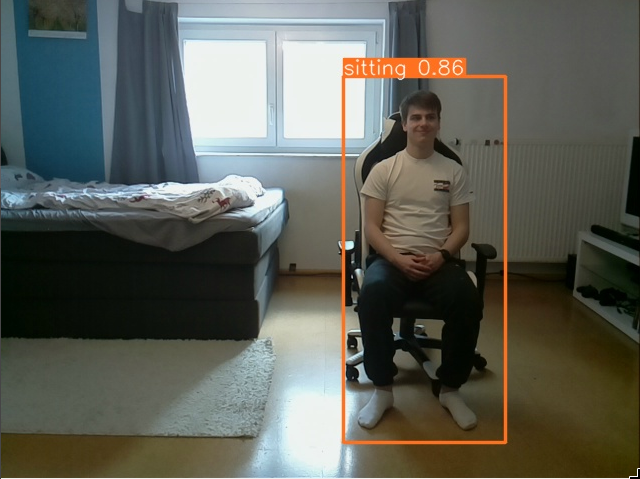
\includegraphics[width=\textwidth]{images/sitting.png}
		\caption*{Klasse: ''sitting''}
	\end{minipage}
	\hfill
	\begin{minipage}[b]{0.3\textwidth}
		\centering
		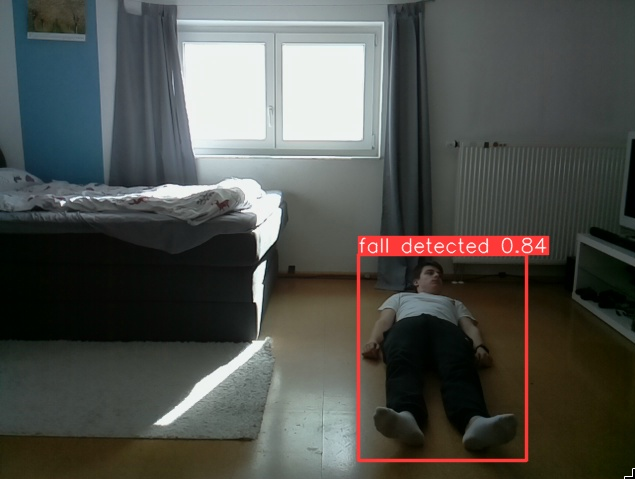
\includegraphics[width=\textwidth]{images/fallen.png}
		\caption*{Klasse: ''fall detected''}
	\end{minipage}
	\caption{YOLOv5 Detektion Klassen}
	\label{fig:yolo_classes}
\end{figure}


Zum Labeln der Daten wurde Makesense.ai verwendet, eine Webseite für das Labeln von Bildern, die es Benutzern ermöglicht, Bilder hochzuladen und Annotationen wie Bounding Boxes und Klassifizierungen hinzuzufügen, um Datensätze für Computer Vision-Anwendungen vorzubereiten \cite{noauthor_make_nodate}. Der Entwickler hat die Daten in drei Klassen unterteilt: 'walking', 'sitting' und 'fall detected' (sieh Abbildung \ref{fig:yolo_classes}).


Das Modell soll dem Entwickler zufolge eine Genauigkeit von 85 bis 90\% bei Tageslicht haben. Es hat jedoch Schwierigkeiten mit der Detektion von vielen Personen auf einem Bild, was zu falschen Erkennungen führen kann. Für unseren Anwendungsfall, die Überwachung von Patienten, ist dies jedoch kein Problem, da wir in unseren Bildern normalerweise nur einzelne Patienten haben.


